\documentclass[a4paper]{article}
\usepackage[spanish]{babel}
\usepackage{graphicx}
\usepackage{listings}

%opening
\title{La memoria de las prácticas de IPO1}
\author{Maciej Nalepa, Piotr Maliszewski}

\begin{document}

\maketitle

\section{Introducción}
% objeto y delimitación de la práctica desarrollada
Un trabajo práctico consistente en el desarrollo de un prototipo de aplicación interactiva de escritorio con interfaz gráfica de usuario (GUI) en Java para gestión de camping. La aplicación permite el manejo de un complejo por un usuario registrado en un sistema abstracto cual no está parte de la interfaz y este proyecto.

La GUI está diseñado teniendo en cuenta los aspectos de usabilidad y factores humanos (leyes de Gestalt, empleo de metáforas, selección adecuada de colores y layouts, diseño de formularios, etc.).

\section{Análisis de requisitios}
% básico y en lenguaje natural

\section{Teconología y recursos utilizados}
 librerías usados
La aplicación utiliza JavaSE-1.8, swing y awt. No hay otras dependencias.

Toda la aplicación está desarrollada con Eclipse y WindowBuilder.

\subsection{Ejecución}
% instrucciones para ejecución
Para ejecutar la aplicación sólo ejecuta el fichero $camping.jar$ con JDK Runtime.
\begin{lstlisting}
	java -jar camping.jar
\end{lstlisting}

Los datos para acceder a la aplicación están entrados en la ventana del inicio automáticamente. Si están borrados, utiliza los siguientes:
\begin{lstlisting}
	Usuario:	MyLogin
	Contraseña:	password
\end{lstlisting}

\section{Justificación del diseño de la GUI}
% en base a lo estudiado en teoría

\begin{figure}[h]
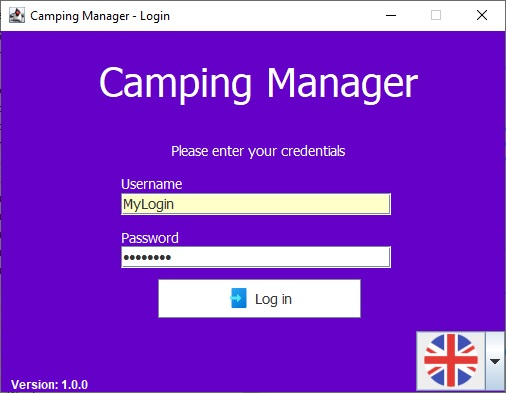
\includegraphics[width=\textwidth]{img/login.jpg}
\caption{Ventana del inicio de sesión}
\end{figure}

\begin{figure}[h]
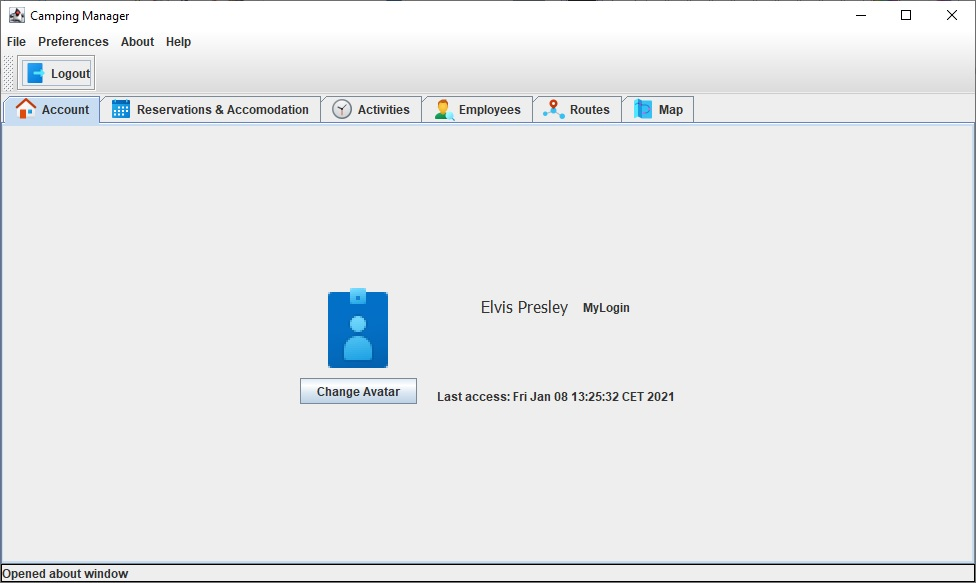
\includegraphics[width=\textwidth]{img/account.jpg}
\caption{Ventana principal}
\end{figure}

\begin{figure}[h]
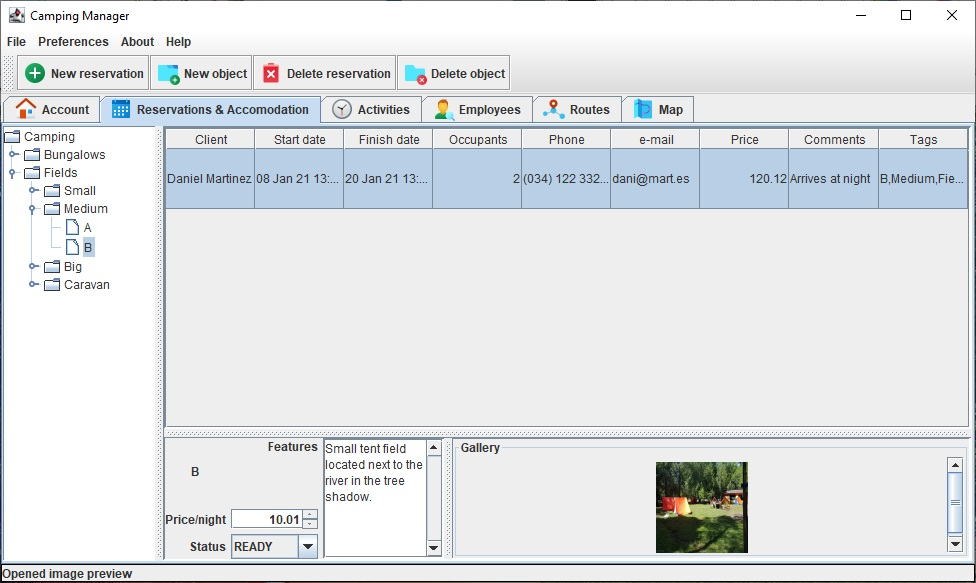
\includegraphics[width=\textwidth]{img/reservation.jpg}
\caption{Manejo de reservas y complejo camping}
\end{figure}
\begin{figure}[h]
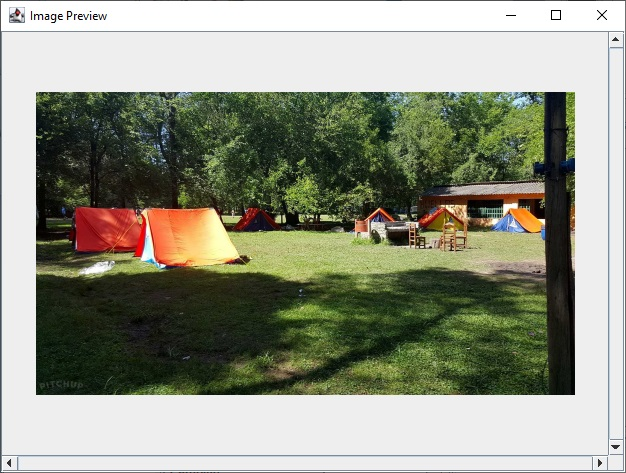
\includegraphics[width=\textwidth]{img/preview.jpg}
\caption{Ventana de la prevista de imagen}
\end{figure}

\begin{figure}[h]
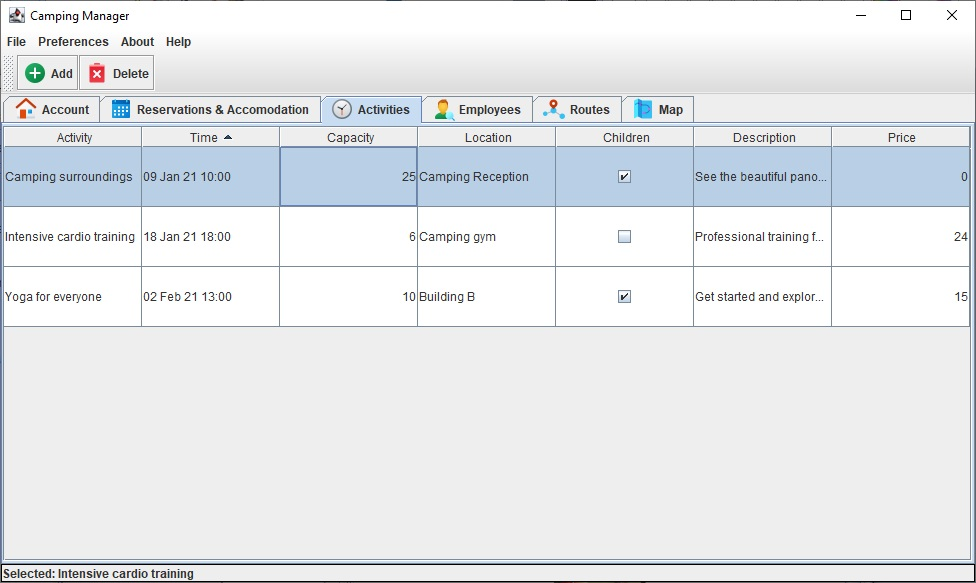
\includegraphics[width=\textwidth]{img/activities.jpg}
\caption{Manejo de actividades}
\end{figure}

\begin{figure}[h]
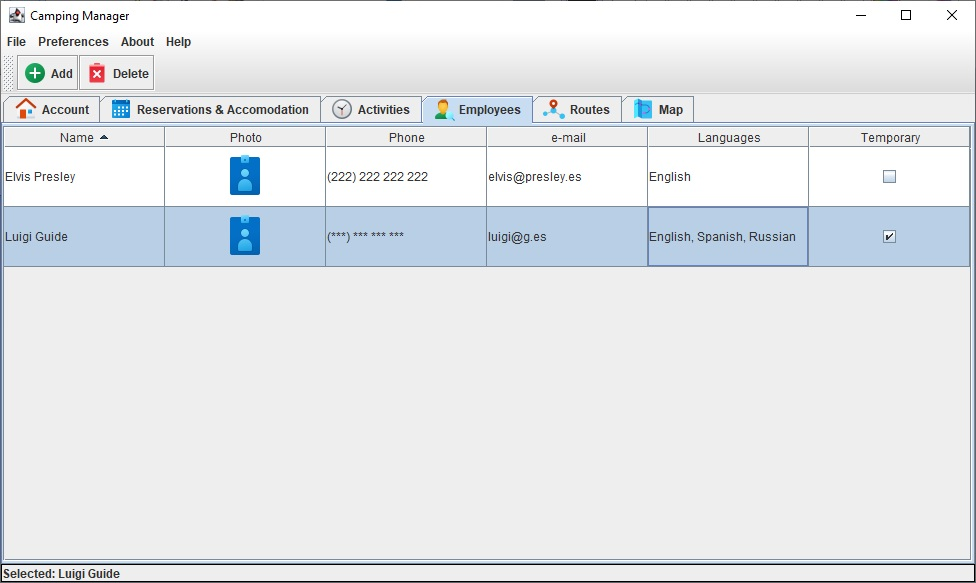
\includegraphics[width=\textwidth]{img/employees.jpg}
\caption{Manejo de empleados}
\end{figure}

\begin{figure}[h]
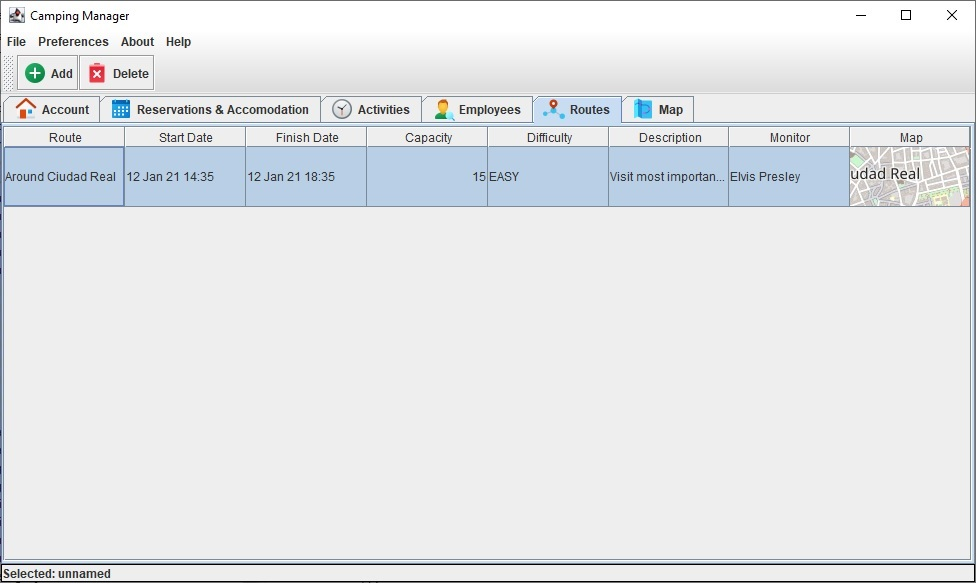
\includegraphics[width=\textwidth]{img/routes.jpg}
\caption{Manejo de rutas}
\end{figure}

\begin{figure}[h]
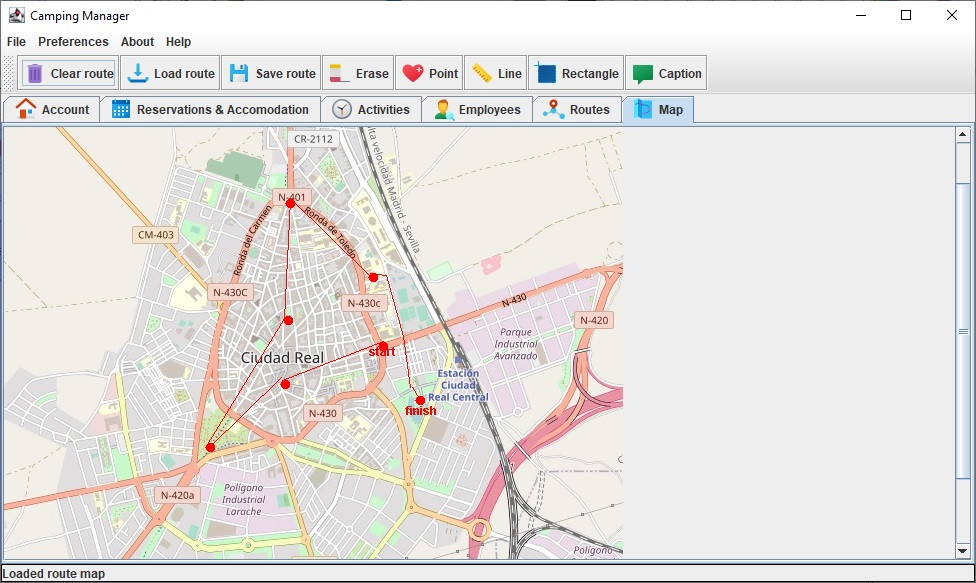
\includegraphics[width=\textwidth]{img/map.jpg}
\caption{Dibujo de las rutas en el mapa}
\end{figure}

\begin{figure}[h]
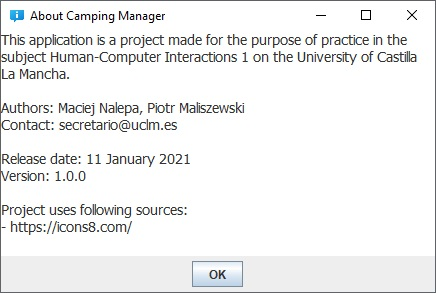
\includegraphics[width=\textwidth]{img/about.jpg}
\caption{Ventana de informaciones sobre la aplicación}
\end{figure}

\begin{figure}[h]
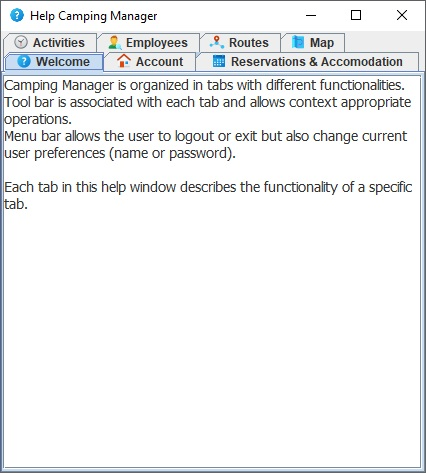
\includegraphics[width=\textwidth]{img/help.jpg}
\caption{Ventana de ayuda}
\end{figure}

\begin{figure}[h]
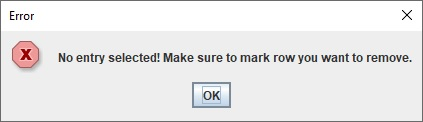
\includegraphics[width=\textwidth]{img/error.jpg}
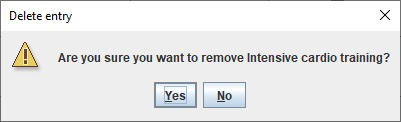
\includegraphics[width=\textwidth]{img/delete-confirmation.jpg}
\caption{Ventanas de mensajes}
\end{figure}

\end{document}

